\documentclass[12pt]{article}
\usepackage{color,amsfonts,amssymb}
\usepackage{amsfonts,epsf,amsmath}
\usepackage{tikz}

\begin{document}

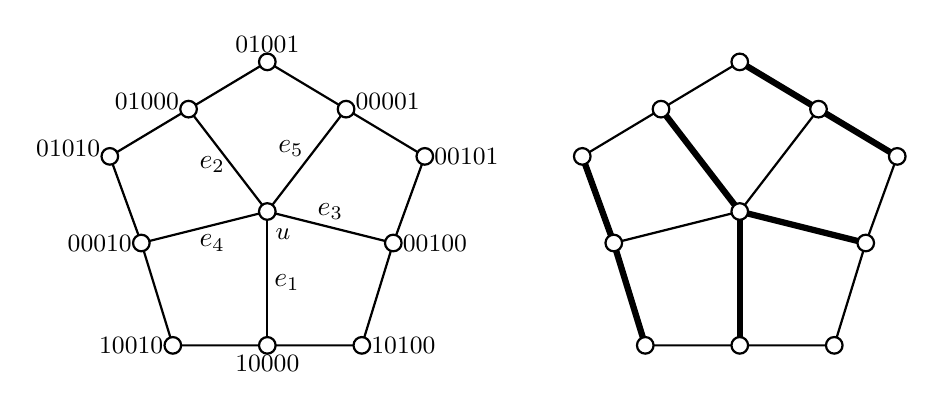
\begin{tikzpicture}[scale=1.0,style=thick]
\def\vr{3pt}

\begin{scope}[xshift=0cm, yshift=0cm]
%% vertices defined %%
\path (0,-0.3) coordinate (u);
\path (0,-2.0) coordinate (x1);
\path (1.6,-0.7) coordinate (x2);
\path (1,1) coordinate (x3);
\path (-1,1) coordinate (x4);
\path (-1.6,-0.7) coordinate (x5);
\path (1.2,-2.0) coordinate (y1);
\path (2.0,0.4) coordinate (y2);
\path (0,1.6) coordinate (y3);
\path (-2.0,0.4) coordinate (y4);
\path (-1.2,-2.0) coordinate (y5);
%% edges %%
\foreach \i in {1,...,5}
{
\draw (u) -- (x\i); 
}
\draw (x1) -- (y1) -- (x2) -- (y2) -- (x3) -- (y3) -- (x4) --(y4) -- (x5) -- (y5) -- (x1); 

%% vertices %%
\draw (u)  [fill=white] circle (\vr);
\foreach \i in {1,...,5}
{
\draw (x\i)  [fill=white] circle (\vr);
\draw (y\i)  [fill=white] circle (\vr);
}
%% text %%
{\small 
\draw[below] (u)++(0.2,-0.1) node {$u$}; 
\draw[below] (x1)++(0.0,0.0) node {$10000$}; 
\draw[right] (x2)++(0.0,0.0) node {$00100$}; 
\draw [right](x3)++(0.0,0.1) node {$00001$}; 
\draw [left](x4)++(0.0,0.1) node {$01000$}; 
\draw[left] (x5)++(0.0,0.0) node {$00010$}; 
}
\draw (0.25,-1.2) node {$e_1$};
\draw (0.8,-0.3) node {$e_3$};
\draw (0.3,0.5) node {$e_5$};
\draw (-0.7,0.3) node {$e_2$};
\draw (-0.7,-0.7) node {$e_4$};
{\small 
\draw[right] (y1)++(0.0,0.0) node {$10100$}; 
\draw[right] (y2)++(0.0,0.0) node {$00101$}; 
\draw [above](y3)++(0.0,0.0) node {$01001$}; 
\draw [left](y4)++(0.0,0.1) node {$01010$}; 
\draw[left] (y5)++(0.0,0.0) node {$10010$}; 
}
\end{scope}

\begin{scope}[xshift=6cm, yshift=0cm]
%% vertices defined %%
\path (0,-0.3) coordinate (u);
\path (0,-2.0) coordinate (x1);
\path (1.6,-0.7) coordinate (x2);
\path (1,1) coordinate (x3);
\path (-1,1) coordinate (x4);
\path (-1.6,-0.7) coordinate (x5);
\path (1.2,-2.0) coordinate (y1);
\path (2.0,0.4) coordinate (y2);
\path (0,1.6) coordinate (y3);
\path (-2.0,0.4) coordinate (y4);
\path (-1.2,-2.0) coordinate (y5);
%% edges %%
\foreach \i in {1,...,5}
{
\draw (u) -- (x\i); 
}
\draw (x1) -- (y1) -- (x2) -- (y2) -- (x3) -- (y3) -- (x4) --(y4) -- (x5) -- (y5) -- (x1); 
\draw[line width=0.8mm] (u) -- (x1); 
\draw[line width=0.8mm] (u) -- (x2); 
\draw[line width=0.8mm] (u) -- (x4); 
\draw[line width=0.8mm] (y5) -- (x5); 
\draw[line width=0.8mm] (x5) -- (y4); 
\draw[line width=0.8mm] (x3) -- (y3); 
\draw[line width=0.8mm] (x3) -- (y2); 
%% vertices %%
\draw (u)  [fill=white] circle (\vr);
\foreach \i in {1,...,5}
{
\draw (x\i)  [fill=white] circle (\vr);
\draw (y\i)  [fill=white] circle (\vr);
}
\end{scope}

\end{tikzpicture}

\end{document}